\documentclass[11pt]{article}

\usepackage[margin=1in]{geometry}
\usepackage[T1]{fontenc}
\usepackage{lmodern}
\usepackage{setspace}
\usepackage{graphicx}
\usepackage{booktabs}
\usepackage{amsmath}
\usepackage{hyperref}
\usepackage{xcolor}
\usepackage{caption}
\usepackage{subcaption}
\usepackage{longtable}
\usepackage{array}
\usepackage{textcomp}
\usepackage{microtype}
\usepackage{lineno}
\usepackage{enumitem}

\setcounter{secnumdepth}{0}

\doublespacing
\linenumbers

\date{}

\begin{document}

%% ============================================================
%% TITLE PAGE
%% ============================================================

\begin{center}
{\Large\bfseries The Power of Open Data: Impact, Equity, and Knowledge Diffusion\\[4pt]
Across Four Major Health Data Repositories}

\vspace{0.6em}
{\small\textit{Running title:} Open Data Impact and Equity}

\vspace{1em}

{\normalsize
Rahul Gorijavolu$^{1,2,3,4,*}$,
Miguel \'Angel Armengol de la Hoz$^{5}$,
Catherine Bielick$^{6}$,
Daniel K. Ebner$^{7}$,
Amelia Fiske$^{8}$,
Jack Gallifant$^{9,10}$,
Judy W. Gichoya$^{11}$,
Nura Izath$^{12}$,
Kaushik Madapati$^{1,2,13}$,
Lucas McCullum$^{14,15}$,
Vishnu Nair$^{3}$,
Milit S Patel$^{2,16}$,
Anna E. Premo$^{17}$,
Alice Rangel Teixeira$^{18}$,
Christopher M. Sauer$^{2,19,20}$,
Leo A. Celi$^{2,21,22}$
}

\vspace{0.8em}

{\scriptsize
$^{1}$AI for Responsible, Generalizable, and Open Surgical (ARGOS) Research Group, Baltimore, MD, USA\\
$^{2}$Laboratory for Computational Physiology, MIT, Cambridge, MA, USA\\
$^{3}$Johns Hopkins University School of Medicine, Baltimore, MD, USA\\
$^{4}$Whiting School of Engineering, Johns Hopkins University, Baltimore, MD, USA\\
$^{5}$Big Data Department, PMC, Fundaci\'on Progreso y Salud, Seville, Spain\\
$^{6}$Division of Infectious Diseases, Beth Israel Deaconess Medical Center, Boston, MA, USA\\
$^{7}$Department of Radiation Oncology, Mayo Clinic, Rochester, MN, USA\\
$^{8}$Institute of History and Ethics in Medicine, TUM School of Medicine and Health, Technical University of Munich, Munich, Germany\\
$^{9}$Artificial Intelligence in Medicine Program, Mass General Brigham, Harvard Medical School, Boston, MA, USA\\
$^{10}$Department of Radiation Oncology, Brigham and Women's Hospital/Dana-Farber Cancer Institute, Boston, MA, USA\\
$^{11}$Department of Radiology and Imaging Sciences, Emory University, Atlanta, GA, USA\\
$^{12}$Mbarara University of Science and Technology Data Science Research Hub (MUDSReH), Mbarara, Uganda\\
$^{13}$College of Engineering, University of California, Berkeley, CA, USA\\
$^{14}$UT MD Anderson Cancer Center UTHealth Houston Graduate School of Biomedical Sciences, Houston, TX, USA\\
$^{15}$Department of Radiation Oncology, UT MD Anderson Cancer Center, Houston, TX, USA\\
$^{16}$Department of Molecular Biosciences, The University of Texas at Austin, Austin, TX, USA\\
$^{17}$Department of Humanities, Social, and Political Science, ETH Zurich, Zurich, Switzerland\\
$^{18}$Department of Philosophy, Universitat Aut\`onoma de Barcelona, Barcelona, Spain\\
$^{19}$Department of Hematology and Stem Cell Transplantation, University Hospital Essen, Essen, Germany\\
$^{20}$Institute for Artificial Intelligence in Medicine, University Hospital Essen, Essen, Germany\\
$^{21}$Division of Pulmonary, Critical Care and Sleep Medicine, Beth Israel Deaconess Medical Center, Boston, MA, USA\\
$^{22}$Department of Biostatistics, Harvard T.H. Chan School of Public Health, Boston, MA, USA\\[6pt]
$^{*}$Corresponding Author: Rahul Gorijavolu, 733 N Broadway, Baltimore, MD 21205, USA.\\
Email: rgorija1@jhmi.edu. Tel: +1 (609) 920-4738.\\[3pt]
Middle authors are listed in alphabetical order by last name.
}
\end{center}

\vspace{1em}

\noindent\textbf{Word count:} Abstract: 349; Main text: ${\sim}$3,800\\
\noindent\textbf{Tables:} 2 \quad \textbf{Figures:} 3 \quad \textbf{Appendix tables:} 3 \quad \textbf{Appendix figures:} 3

\newpage

%% ============================================================
%% STRUCTURED ABSTRACT
%% ============================================================

\noindent\textbf{\large Abstract}

\vspace{0.5em}

\noindent\textbf{Background}\quad
Open health data repositories receive billions in public funding, yet no systematic framework exists to evaluate their downstream scholarly impact, the equity of the research communities they cultivate, or the breadth of disciplines they reach. We introduce a two-degree citation methodology to quantify knowledge diffusion from open data, normalized by funding, and apply it to four major health data repositories.

\noindent\textbf{Methods}\quad
Using the OpenAlex bibliometric database (February 2026), we identified all first-degree citing publications (\textit{n}\,=\,30,049) and their second-degree citers (\textit{n}\,=\,485,396) for MIMIC (versions I--IV; retrospective EHR data; \$14.4M), UK Biobank (prospective cohort with genomics; \$525.5M), OpenSAFELY (federated EHR platform; \$53.7M), and All of Us (prospective national cohort with biobanking and community engagement; \$2,160M). We extracted author demographics (gender via Genderize.io, institutional country income via World Bank 2024 classifications) and research topics. Chi-square tests with odds ratios assessed demographic differences across repositories.

\noindent\textbf{Results}\quad
Funding-normalized first-degree papers per \$1M ranged from 689 (MIMIC) to 1 (All of Us). Citation amplification from first- to second-degree was consistent across repositories (9.3--11.5$\times$). Author demographics differed significantly (\textit{p}\,$<$\,0.001): LMIC authorship ranged from 41.8\% (MIMIC) to 4.3\% (All of Us), while female authorship showed an inverse pattern (31.8\% to 43.2\%). Female authors were consistently underrepresented in senior (last-author) compared with first-author positions across all repositories. Differences in scope, design, and what funding covers limit direct comparisons.

\noindent\textbf{Conclusions}\quad
Open health data generates a consistent ${\sim}$10$\times$ indirect citation amplification beyond its direct users. However, citation-based metrics favor datasets adopted as computational benchmarks and cannot capture clinical translation, capacity building, or community engagement. The large differences in funding-normalized output partly reflect structural differences between retrospective databases and prospective cohorts. A complete assessment of open data investments requires examining the research communities and knowledge ecosystems these repositories cultivate, including who is producing the research and from where.

\vspace{1em}

\noindent\textbf{Keywords:} open data; bibliometrics; citation analysis; health data repositories; research equity; knowledge diffusion

\newpage

%% ============================================================
%% KEY MESSAGES BOX
%% ============================================================

\begin{center}
\fbox{\parbox{0.9\textwidth}{
\textbf{What is already known on this topic}
\begin{itemize}[nosep,leftmargin=*]
\item Open health data repositories receive public funding ranging from millions to billions of dollars, with mandates for open access increasing globally.
\item Existing evaluations count direct publications or citations but do not capture the broader downstream knowledge diffusion from open data.
\item Demographic disparities in scientific authorship are well documented, but their relationship to specific data repositories has not been systematically examined.
\end{itemize}

\vspace{0.5em}
\textbf{What this study adds}
\begin{itemize}[nosep,leftmargin=*]
\item A two-degree citation methodology reveals that each open health data repository generates a consistent ${\sim}$10$\times$ indirect citation amplification, regardless of repository type or funding scale.
\item MIMIC has the highest LMIC authorship (41.8\%) but lowest female authorship (31.8\%); this gender gap is explained by its dominant citing discipline being computer science (43.1\%) rather than medicine.
\item Women are underrepresented in senior authorship positions relative to first-author positions across all four repositories, with the gap ranging from 4.9 to 10.9 percentage points.
\end{itemize}

\vspace{0.5em}
\textbf{How this study might affect research, practice, or policy}
\begin{itemize}[nosep,leftmargin=*]
\item Funders should incorporate indirect (second-degree) citation impact when evaluating open data investments, as first-degree metrics capture only ${\sim}$10\% of the scholarly footprint.
\item Addressing gender gaps in open data communities may require disciplinary-level interventions (e.g., in computer science) rather than changes to data access policies alone.
\item High LMIC authorship on a dominant dataset does not guarantee equitable participation; evaluations should examine whether LMIC researchers hold senior authorship positions and whether local datasets receive comparable investment.
\end{itemize}
}}
\end{center}

\newpage

%% ============================================================
\section{Introduction}
\label{sec:introduction}
%% ============================================================

Open data sharing has become a cornerstone of biomedical research policy.
Major funding agencies including the U.S. National Institutes of Health [1] and the Wellcome Trust [2] now mandate that publicly funded datasets be made accessible, reflecting a growing consensus that open data accelerates scientific discovery [3,4].
This commitment has translated into substantial public investment: in health sciences alone, programs such as the All of Us Research Program (\$2.16 billion) [5], UK Biobank (\textsterling 413.8 million) [6], and the MIMIC critical care database (\$14.4 million) [7] span orders of magnitude in funding yet share the common goal of enabling secondary research.

Despite these investments, there is no systematic framework for evaluating not only the downstream scholarly impact of open health data repositories, but also \textit{who} comprises the research communities they cultivate.
Existing bibliometric evaluations typically count publications or first-degree citations --- papers that directly use a dataset --- but fail to capture the broader knowledge diffusion that occurs when those papers are themselves cited by others [8,9].
This indirect ``ripple'' effect is critical because the value of open data extends well beyond its immediate users: a clinical prediction model built on MIMIC may be cited by implementation science researchers, health economists, or computer scientists who never access the original data.

Equally important is the question of equity.
Global disparities in scientific publishing are well documented [10], and open data has been proposed as a mechanism for leveling the playing field by providing researchers in low- and middle-income countries (LMICs) access to datasets they could not independently generate [11].
Yet whether this promise is being realized --- and whether open data attracts diverse researchers into positions of intellectual leadership, not merely participation --- remains an empirical question.
Understanding \textit{who} does the research, \textit{where} they are located, and \textit{what positions} they hold in the authorship hierarchy is as important as counting how many papers a dataset generates.

In this study, we introduce a two-degree citation methodology that traces both direct citations (first-degree: papers that use a dataset) and indirect citations (second-degree: papers citing those first-degree papers) to quantify knowledge diffusion from open data, normalized by cumulative program funding.
We apply this framework to four major open health data repositories spanning different designs, maturity stages, and funding scales: MIMIC (versions I--IV; retrospective electronic health records) [7,12], UK Biobank (a prospective population cohort with genomic data) [6,13], OpenSAFELY (a federated analytics platform for primary care records) [14], and All of Us (a prospective national cohort emphasizing participant diversity) [5,15].

Our objectives are threefold: (1) to quantify funding-normalized scholarly output at both degrees of citation, (2) to characterize the demographics of the research communities each repository has cultivated --- including gender representation, geographic diversity, and authorship position --- and (3) to examine how equity patterns vary across repositories that serve fundamentally different research communities.


%% ============================================================
\section{Methods}
\label{sec:methods}
%% ============================================================

\subsection{Study Design}

This is a cross-sectional bibliometric analysis of four open health data repositories.
No human participants were involved, and no ethics approval was required.

\subsection{Data Repositories}
\label{sec:repositories}

We selected four open health data repositories representing distinct models of data sharing in biomedicine (Table~\ref{tab:overview}).

\textbf{MIMIC} (Medical Information Mart for Intensive Care) is a family of freely accessible critical care databases originating from Beth Israel Deaconess Medical Center.
MIMIC-I was first released in 1997 [16], with subsequent versions (II, III, IV) expanding in scope and detail [7,12].
MIMIC is a retrospective database built from routinely collected EHR data; its total estimated funding is \$14.4 million.

\textbf{UK Biobank} is a prospective cohort study of approximately 500,000 participants aged 40--69, with data available for approved research since 2015 [6].
The resource includes genotyping, imaging, and longitudinal health outcomes, with cumulative funding of approximately \$525.5 million [13].

\textbf{OpenSAFELY} is a secure, federated analytics platform providing access to de-identified primary care records of approximately 58 million patients in England [14].
Launched during the COVID-19 pandemic in 2020, it has received approximately \$53.7 million in grant funding [17].

\textbf{All of Us} is a longitudinal research program of the U.S. National Institutes of Health aiming to enroll one million or more participants reflecting the diversity of the United States [5].
Its funding encompasses participant recruitment, biobanking, genomic sequencing, return of results, and community engagement infrastructure, totaling approximately \$2.16 billion [15].

These repositories differ fundamentally in what their funding covers.
MIMIC's budget supports curation of data that already exists in hospital systems; All of Us's budget funds prospective recruitment, biospecimen collection, community advisory boards, and return of genomic results.
These structural differences are essential context for interpreting funding-normalized comparisons.

\subsection{Citation Data Collection}
\label{sec:citation-collection}

Using the OpenAlex bibliometric database [18], we identified all publications citing each repository's primary works (retrieved February 2026).
For MIMIC, we combined citations across all four versions (I--IV) and deduplicated by OpenAlex work identifier.
These citing publications constitute the \textit{first-degree} corpus.
We then retrieved all publications citing these first-degree papers, forming the \textit{second-degree} corpus.
In total, we identified 30,049 first-degree and 485,396 second-degree publications.

\subsection{Author Demographics}
\label{sec:demographics}

Author gender was inferred from first names using the Genderize.io API [19], which returns probabilistic gender assignments based on a global name--gender database.
The identification rate exceeded 98\% across all repositories.

Institutional country was determined from author affiliation metadata in OpenAlex.
Countries were classified as high-income (HIC) or low- and middle-income (LMIC) using the World Bank 2024 income classification [20].
HIC--LMIC collaboration was defined as any publication with authors from both income groups.

We analyzed authorship positions separately: first authors (typically the primary researcher), last authors (typically the senior or supervising investigator), and middle authors.
This distinction is important because first- and last-author positions carry different implications for intellectual leadership, career advancement, and mentorship roles within research teams.

Name-based gender inference has known limitations: it performs poorly for some cultural contexts, conflates gender identity with name-associated gender, and cannot capture non-binary identities.
Institutional affiliation may not reflect nationality or career trajectory.
These proxies are standard in large-scale bibliometric analyses but should be interpreted as approximations.

\subsection{Disciplinary Analysis}
\label{sec:disciplinary}

OpenAlex assigns each publication a hierarchical topic classification.
We extracted the primary field assignment for each first-degree publication and computed field proportions by repository and year.
Full disciplinary diffusion results are reported in the Appendix (eFigure~1).

\subsection{Statistical Analysis}
\label{sec:statistical}

Differences in author demographics across repositories were assessed using Pearson's chi-square tests, with Cram\'{e}r's $V$ as the effect size.
Pairwise comparisons between MIMIC and each other repository used chi-square tests with Bonferroni correction ($n = 3$).
Odds ratios (OR) with 95\% confidence intervals were computed for all $2 \times 2$ comparisons.
The significance level was set at $\alpha = 0.05$.

Funding-normalized metrics were computed by dividing raw counts by total program funding in millions of U.S. dollars.
The citation amplification ratio was defined as the ratio of total second-degree citation mass to total first-degree citation mass for each repository.

\subsection{Patient and Public Involvement}

Patients and the public were not involved in the design, conduct, or reporting of this bibliometric analysis.


%% ============================================================
\section{Results}
\label{sec:results}
%% ============================================================

\subsection{Citation Output and Funding-Normalized Impact}
\label{sec:results-citations}

Table~\ref{tab:overview} summarizes the citation output and funding context for each repository.
First-degree papers ranged from 2,066 (All of Us) to 11,803 (UK Biobank).
When normalized by funding, the variation was far more pronounced: MIMIC generated 689 first-degree papers per \$1 million, compared with 116 (OpenSAFELY), 22 (UK Biobank), and 1 (All of Us).

This pattern amplified at the second degree.
MIMIC's 118,904 second-degree papers translated to 8,257 per \$1 million, versus 2,314 (OpenSAFELY), 405 (UK Biobank), and 14 (All of Us).
The cumulative second-degree citation mass per \$1 million was 141,752 for MIMIC and 177 for All of Us, an approximately 800-fold difference.

Despite this wide variation, the citation amplification ratio was remarkably consistent: 9.3$\times$ (MIMIC), 11.5$\times$ (UK Biobank), 10.8$\times$ (OpenSAFELY), and 10.8$\times$ (All of Us).
This ${\sim}$10$\times$ multiplier indicates that the indirect scholarly footprint of open data is approximately an order of magnitude larger than its direct footprint, regardless of repository type or funding scale.

Figure~\ref{fig:cumulative} shows the cumulative growth in first-degree papers over time, and Figure~\ref{fig:ripple} presents funding-normalized first- and second-degree counts side by side.
Figure~\ref{fig:iceberg} visualizes the cumulative funding-normalized citation trajectory as an ``iceberg'' plot, with first-degree citations above and second-degree citations below, illustrating the persistent ${\sim}$10$\times$ amplification ratio across all repositories.

\begin{table}[htbp]
\centering
\caption{Repository characteristics, citation output, and author demographics. Funding figures represent total program investment to date. First-degree papers are publications directly citing a repository's primary works; second-degree papers cite those first-degree papers. Author demographics are computed across all first-degree publications. Gender was inferred via Genderize.io (identification rate $>$98\% for all repositories). Country income classification follows World Bank 2024 definitions.}
\label{tab:overview}
\small
\begin{tabular}{@{}lcccc@{}}
\toprule
& \textbf{MIMIC} & \textbf{UK Biobank} & \textbf{OpenSAFELY} & \textbf{All of Us} \\
\midrule
\multicolumn{5}{l}{\textit{Repository Characteristics}} \\[3pt]
Design & Retrospective EHR & Prospective cohort & Federated EHR & Prospective cohort \\
First data release & 1997 & 2015 & 2020 & 2018 \\
Total funding (\$M) & 14.4 & 525.5 & 53.7 & 2,160 \\
\midrule
\multicolumn{5}{l}{\textit{Citation Output}} \\[3pt]
1st-degree papers & 9,924 & 11,803 & 6,256 & 2,066 \\
2nd-degree papers & 118,904 & 212,737 & 124,285 & 29,470 \\
1st-degree per \$1M & 689 & 22 & 116 & 1 \\
2nd-degree per \$1M & 8,257 & 405 & 2,314 & 14 \\
Amplification ratio & 9.3$\times$ & 11.5$\times$ & 10.8$\times$ & 10.8$\times$ \\
\midrule
\multicolumn{5}{l}{\textit{Author Demographics}} \\[3pt]
Total authors & 57,713 & 126,115 & 70,043 & 21,483 \\
Unique authors & 33,573 & 51,783 & 44,441 & 13,238 \\
Female (\%) & 31.8 & 38.6 & 41.7 & 43.2 \\
Countries represented & 105 & 134 & 148 & 91 \\
LMIC authors (\%) & 41.8 & 22.9 & 17.4 & 4.3 \\
HIC--LMIC collab.\ (\%) & 11.8 & 16.4 & 12.1 & 8.4 \\
\bottomrule
\end{tabular}
\end{table}


\begin{figure}[htbp]
\centering
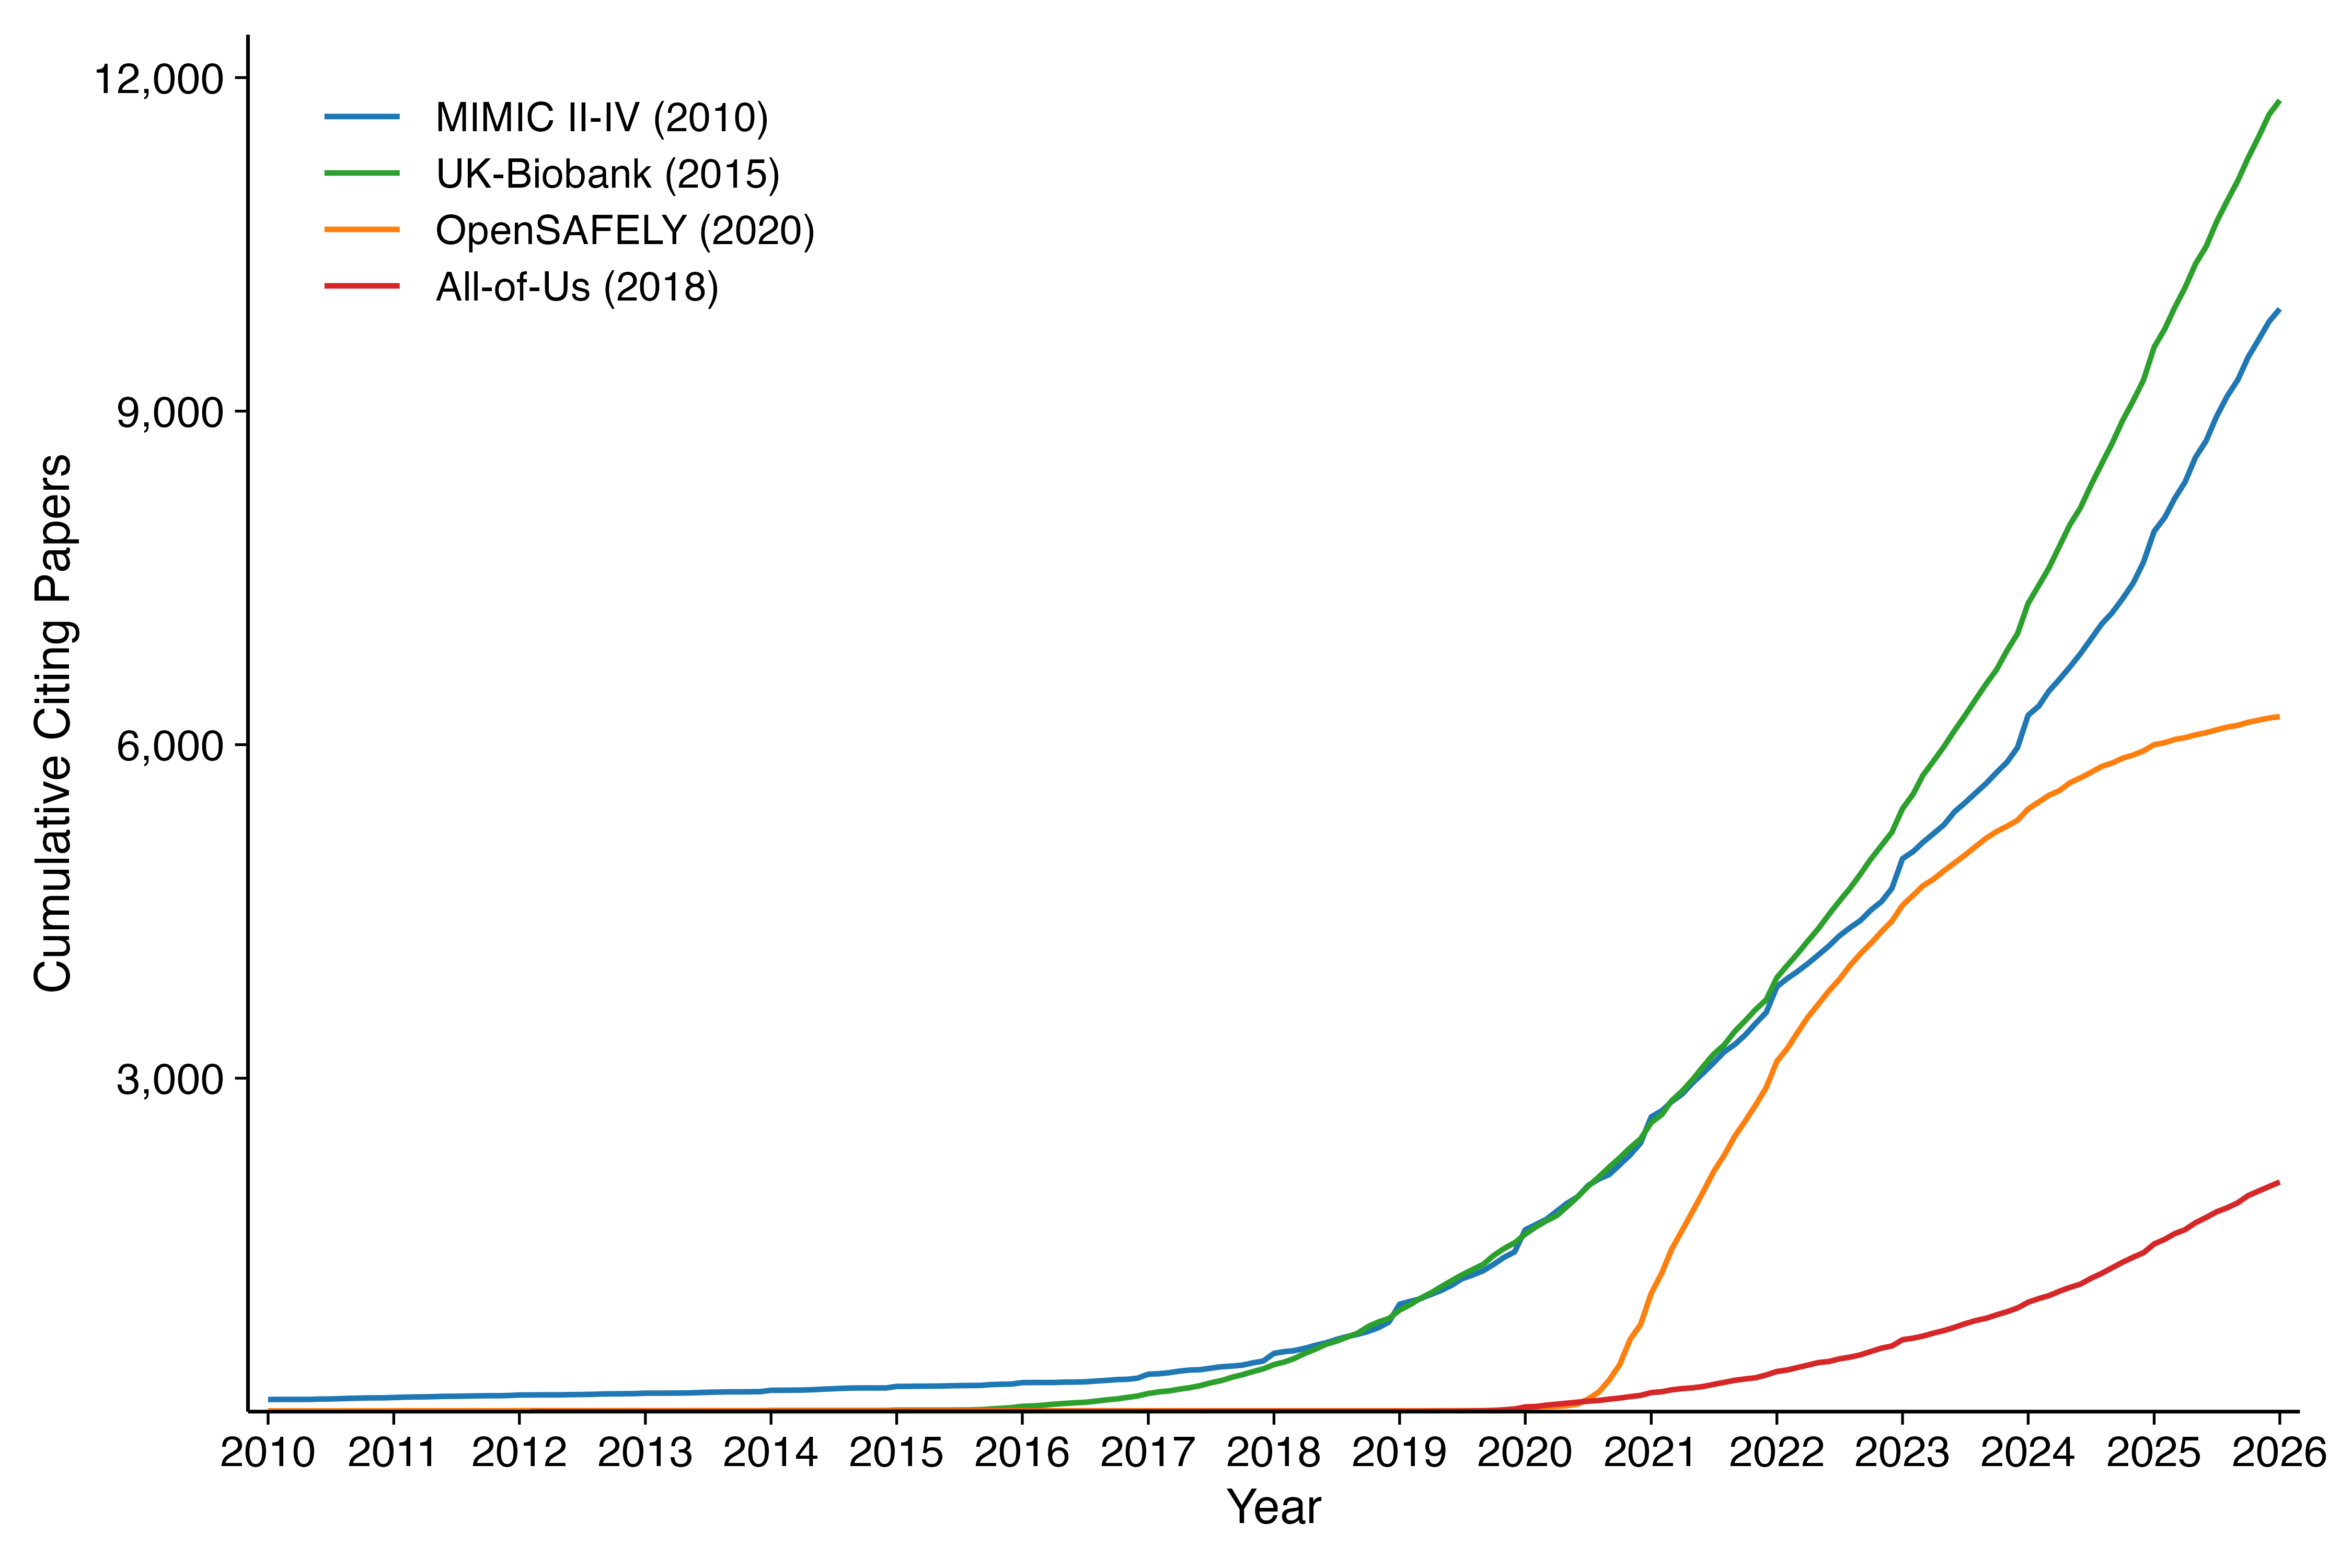
\includegraphics[width=\textwidth]{figures/fig1_cumulative_citations.png}
\caption{Cumulative first-degree publications over time for each repository (monthly resolution). Year of first data availability is shown in parentheses.}
\label{fig:cumulative}
\end{figure}

\begin{figure}[htbp]
\centering
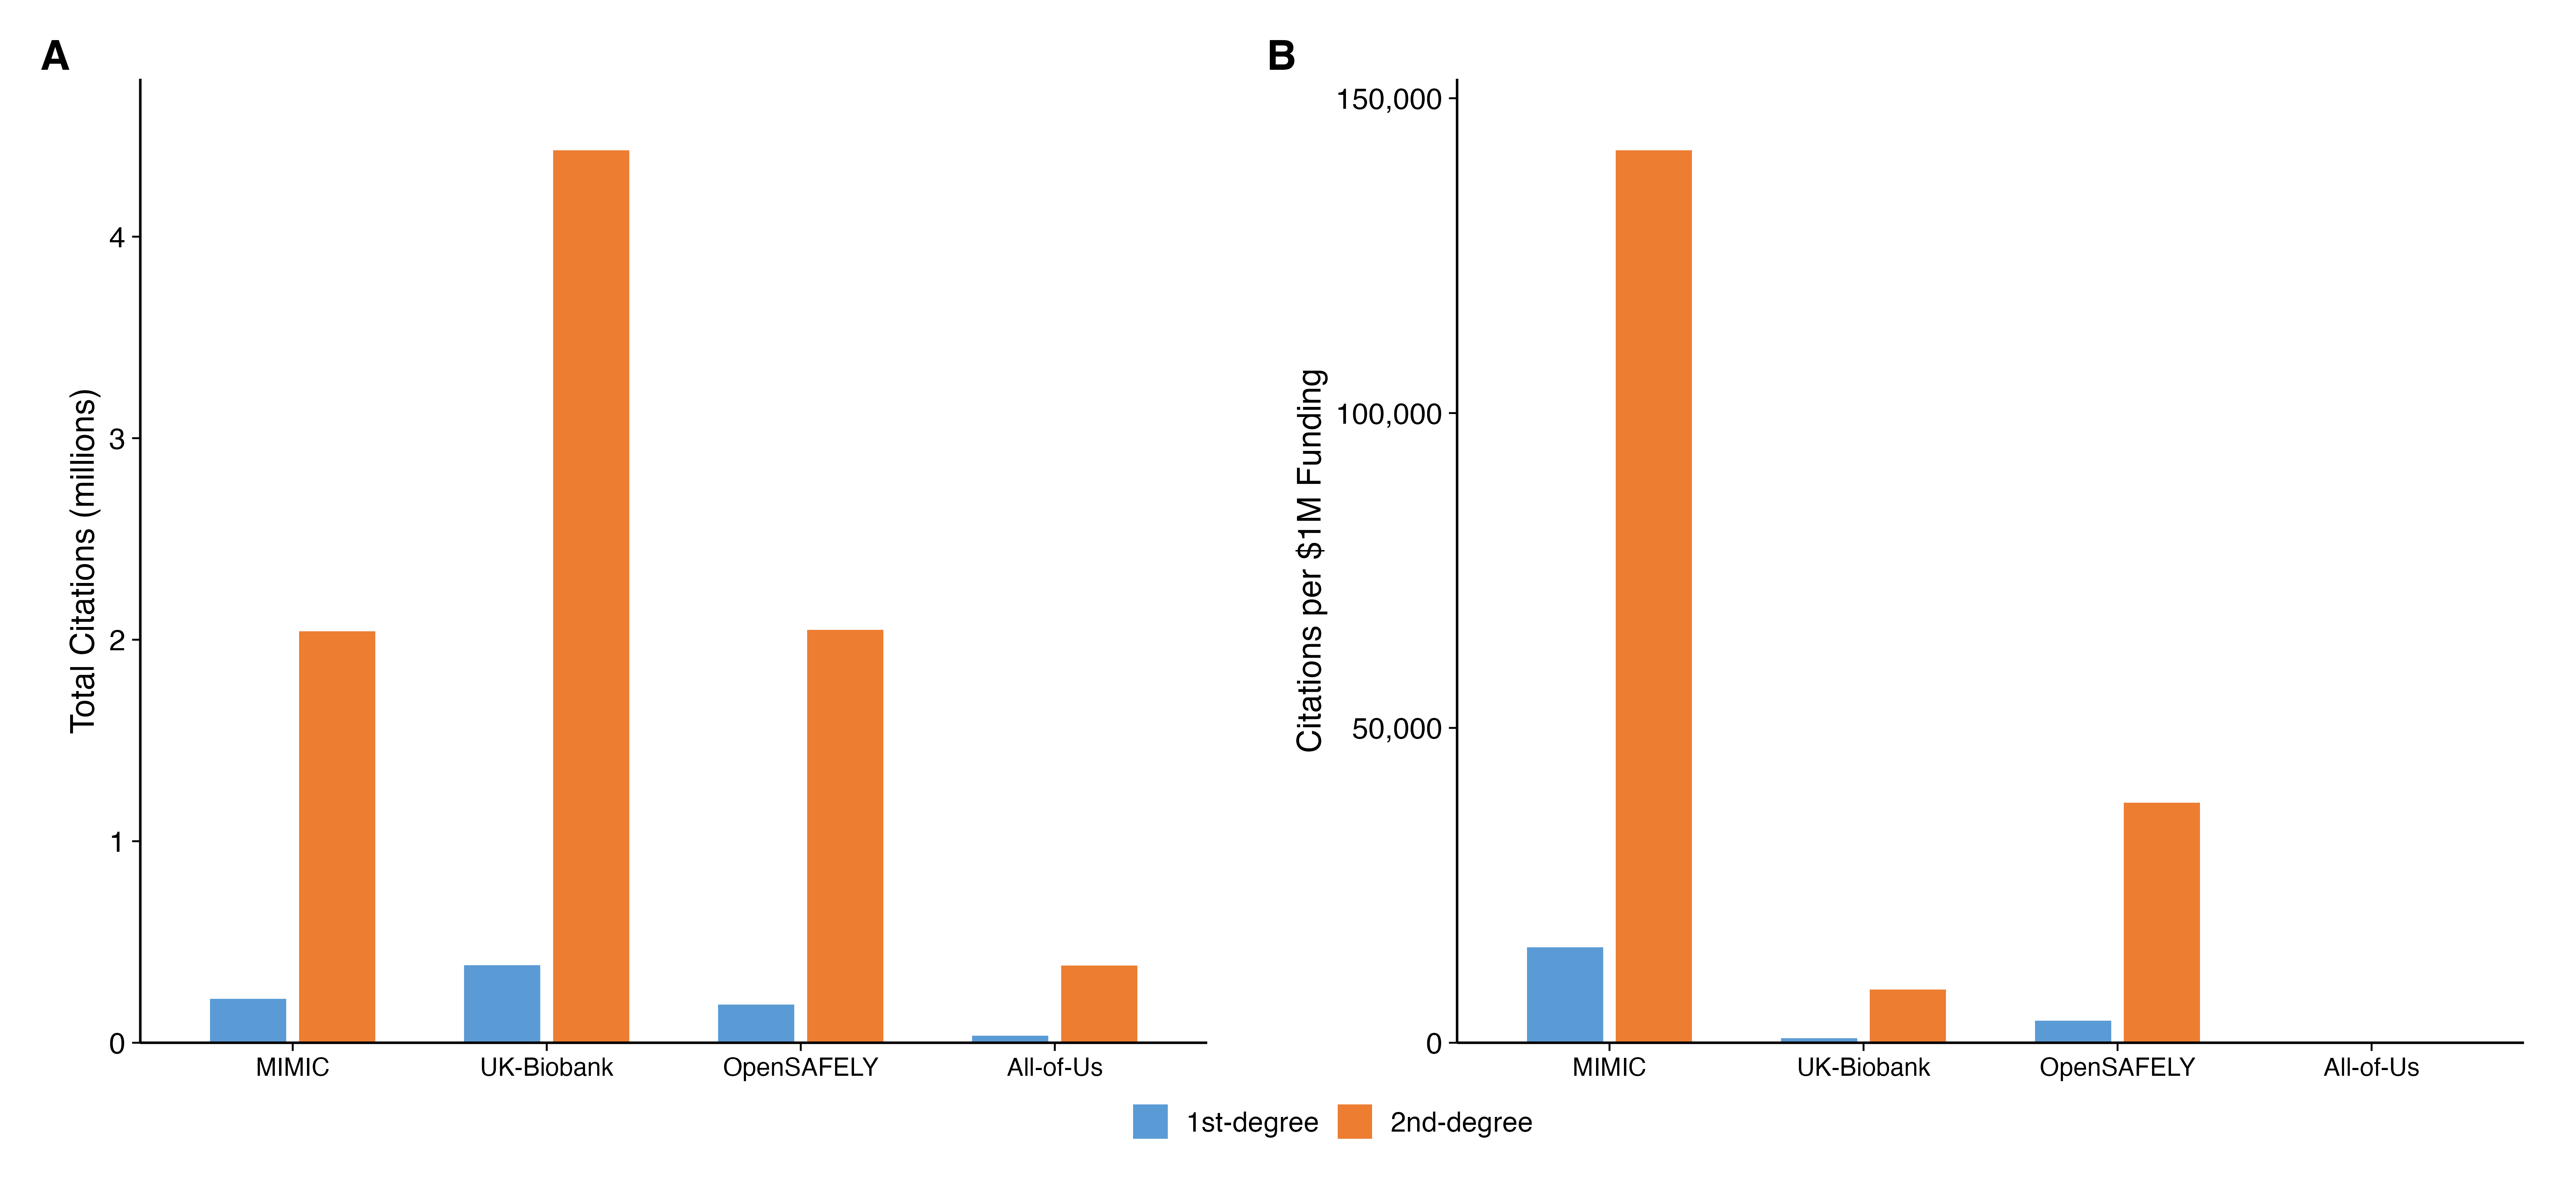
\includegraphics[width=\textwidth]{figures/fig2_funding_normalized_ripple.png}
\caption{First-degree and second-degree citation counts, absolute (left) and normalized per \$1 million in funding (right).}
\label{fig:ripple}
\end{figure}

\begin{figure}[htbp]
\centering
\includegraphics[width=\textwidth]{figures/fig3_iceberg_over_time.png}
\caption{Cumulative funding-normalized citation trajectories. Top panel: first-degree (direct) citations per \$1M. Bottom panel: second-degree (indirect) citations per \$1M. Panel heights are proportional to maximum values. Note different y-axis scales.}
\label{fig:iceberg}
\end{figure}


\subsection{Who Is Doing the Research: Author Demographics and Equity}
\label{sec:results-equity}

Table~\ref{tab:demographics} presents the full demographic profile of research communities across repositories, including authorship position analysis.

\subsubsection{Geographic Diversity and LMIC Representation}

Author demographics differed significantly across all four repositories for LMIC representation ($\chi^2 = 14{,}435.2$, $df = 3$, $p < 0.001$, $V = 0.247$).
MIMIC had the highest proportion of LMIC-affiliated authors (41.8\%), followed by UK Biobank (22.9\%), OpenSAFELY (17.4\%), and All of Us (4.3\%).
The contrast was stark: MIMIC's odds of LMIC authorship were 17.7 times those of All of Us (OR $= 17.71$, 95\% CI 16.45--19.07; $p < 0.001$).

Research citing these repositories originated from 91 (All of Us) to 148 (OpenSAFELY) countries.
However, geographic breadth did not correspond with LMIC depth: OpenSAFELY drew authors from the most countries but had relatively low LMIC representation (17.4\%), reflecting the UK-centric nature of its primary care data.
HIC--LMIC collaboration rates ranged from 8.4\% (All of Us) to 16.4\% (UK Biobank).

Critically, MIMIC's high LMIC authorship extended to positions of intellectual leadership.
LMIC researchers comprised 43.8\% of first authors and 41.5\% of last (senior) authors on MIMIC-citing papers, compared with just 4.1\% and 3.0\% for All of Us, respectively.
This suggests that LMIC researchers are not merely participating in MIMIC's research ecosystem as middle authors but are leading studies and serving as senior investigators.

\subsubsection{Gender Representation}

Gender distribution also differed significantly across repositories ($\chi^2 = 1{,}583.9$, $df = 3$, $p < 0.001$, $V = 0.076$), but the pattern was inverted relative to LMIC authorship.
Female authorship was lowest for MIMIC (31.8\%) and highest for All of Us (43.2\%), with UK Biobank (38.6\%) and OpenSAFELY (41.7\%) between.
MIMIC's odds of female authorship were significantly lower than all comparators (OR $= 0.61$ vs.\ All of Us, 95\% CI 0.59--0.63; OR $= 0.65$ vs.\ OpenSAFELY; OR $= 0.74$ vs.\ UK Biobank; all $p < 0.001$).

\subsubsection{The Senior Authorship Gap}

A consistent pattern emerged across all four repositories: women were better represented in first-author positions than in last-author (senior) positions.
The gap ranged from 4.9 percentage points (MIMIC: 32.3\% first vs.\ 27.4\% last; OR $= 1.27$, $p < 0.001$) to 10.9 percentage points (UK Biobank: 42.2\% vs.\ 31.3\%; OR $= 1.61$, $p < 0.001$).
OpenSAFELY (43.0\% vs.\ 34.6\%; OR $= 1.43$, $p < 0.001$) and All of Us (42.7\% vs.\ 37.6\%; OR $= 1.24$, $p = 0.001$) showed intermediate gaps.

This first-to-last-author gradient indicates that while women are increasingly represented as primary researchers, the transition to senior or supervisory roles --- which typically carry greater influence over research agendas, mentorship, and resource allocation --- remains unequal across all open health data communities.

\subsubsection{Intersectional Patterns}

Intersectional analysis (eTable~2) revealed that LMIC-affiliated female authors had higher representation within the LMIC subgroup than HIC-affiliated female authors had within the HIC subgroup.
For example, among MIMIC first authors, 36.4\% of LMIC authors were female compared with 30.0\% of HIC authors.
This pattern held across all repositories, suggesting that the LMIC research workforce engaging with open health data is, if anything, more gender-balanced than its HIC counterpart.

\begin{table}[htbp]
\centering
\caption{Author demographics and authorship position analysis across repositories. Gender was inferred via Genderize.io (identification rate $>$98\% for all repositories). Country income classification follows World Bank 2024 definitions. HIC--LMIC collaboration indicates publications with authors from both income groups. First and last author positions are analyzed separately to distinguish primary researchers from senior investigators.}
\label{tab:demographics}
\small
\begin{tabular}{@{}lcccc@{}}
\toprule
& \textbf{MIMIC} & \textbf{UK Biobank} & \textbf{OpenSAFELY} & \textbf{All of Us} \\
\midrule
\multicolumn{5}{l}{\textit{Overall Author Demographics}} \\[3pt]
Total author records & 57,713 & 126,115 & 70,043 & 21,483 \\
Unique authors & 33,573 & 51,783 & 44,441 & 13,238 \\
Countries represented & 105 & 134 & 148 & 91 \\
Female authors (\%) & \textbf{31.8} & 38.6 & 41.7 & 43.2 \\
LMIC authors (\%) & \textbf{41.8} & 22.9 & 17.4 & 4.3 \\
HIC--LMIC collab.\ (\%) & 11.8 & 16.4 & 12.1 & 8.4 \\
\midrule
\multicolumn{5}{l}{\textit{First Author Position}} \\[3pt]
Female first authors (\%) & 32.3 & 42.2 & 43.0 & 42.7 \\
LMIC first authors (\%) & \textbf{43.8} & 29.4 & 22.0 & 4.1 \\
\midrule
\multicolumn{5}{l}{\textit{Last Author (Senior) Position}} \\[3pt]
Female last authors (\%) & 27.4 & 31.3 & 34.6 & 37.6 \\
LMIC last authors (\%) & \textbf{41.5} & 26.7 & 21.9 & 3.0 \\
\midrule
\multicolumn{5}{l}{\textit{Statistical Comparisons}} \\[3pt]
\multicolumn{5}{l}{Gender: $\chi^2 = 1{,}583.9$, $df = 3$, $p < 0.001$, $V = 0.076$} \\
\multicolumn{5}{l}{LMIC: $\chi^2 = 14{,}435.2$, $df = 3$, $p < 0.001$, $V = 0.247$} \\
\bottomrule
\end{tabular}

\vspace{4pt}
{\footnotesize Boldface indicates highest value in each row. OR for LMIC (MIMIC vs.\ All of Us) $= 17.71$ (95\% CI 16.45--19.07). OR for female authorship (MIMIC vs.\ All of Us) $= 0.61$ (95\% CI 0.59--0.63). All pairwise comparisons $p < 0.001$ after Bonferroni correction. Full pairwise results in eTable~1.}
\end{table}



%% ============================================================
\section{Discussion}
\label{sec:discussion}
%% ============================================================

\subsection{Principal Findings}

This study introduces a two-degree citation methodology to evaluate the scholarly impact and equity of four major open health data repositories.
Three principal findings emerge: (1) a consistent ${\sim}$10$\times$ citation amplification from direct to indirect citations, (2) stark differences in who comprises each repository's research community, with an inverse relationship between LMIC representation and female authorship, and (3) a persistent gender gap in senior authorship across all repositories.

\subsection{The Research Communities Behind Open Data}

The most consequential finding may not be the citation counts but rather the composition of the communities producing the research.
MIMIC's research ecosystem is distinctive: 41.8\% LMIC authorship, researchers from 105 countries, and --- crucially --- LMIC researchers holding first- and last-author positions at rates comparable to their overall representation.
This suggests that MIMIC has cultivated a research community where LMIC investigators exercise genuine intellectual leadership, not merely participation.

Several structural features may explain this pattern.
MIMIC is freely accessible with no financial barrier, requires only an online training course for credentialing, and operates on data small enough to be downloaded and analyzed on a personal computer.
The extensive datathon program, which has engaged researchers at events in over 30 countries, provides hands-on mentorship and entry into collaborative networks.
These features lower multiple barriers simultaneously: cost, infrastructure, and social capital.

By contrast, All of Us's 4.3\% LMIC authorship reflects the program's design as a U.S.-focused cohort.
Its data use agreements, institutional requirements, and analysis platform may present barriers for international researchers.
UK Biobank and OpenSAFELY, while drawing from more countries, also show relatively modest LMIC authorship (22.9\% and 17.4\%), consistent with their UK-centric data and governance structures.

However, high LMIC authorship on a dominant dataset does not automatically indicate equitable participation.
LMIC researchers using MIMIC produce research legible to Global North journals, which benefits their careers but may not translate into equivalent investment in building open datasets within their own health systems [11].
True equity would include LMIC-generated datasets achieving comparable citation amplification.

\subsection{The Gender Gap: A Disciplinary, Not Data Access, Problem}

MIMIC's low female authorship (31.8\%) initially appears paradoxical given its otherwise equitable access model.
However, MIMIC is the only repository whose primary citing field is computer science (43.1\% of papers; see eFigure~1) rather than medicine.
The gender gap in computer science authorship is well documented [10,23], and MIMIC's female authorship rate is consistent with the field's broader demographics rather than a barrier intrinsic to the dataset.

The persistent senior authorship gap --- women were 5--11 percentage points less represented in last-author than first-author positions across all four repositories --- mirrors well-documented patterns in biomedicine [10,24,25].
This gap transcends individual datasets and reflects structural inequities in career advancement, mentorship, and access to independent funding.
Interventions at the repository level (e.g., modifying data access) are unlikely to address this; systemic changes in academic promotion and mentorship structures are needed.

\subsection{Funding Efficiency in Context}

The approximately 800-fold difference in funding-normalized second-degree citations between MIMIC and All of Us requires careful contextualization.
MIMIC retrospectively curates data that already exists; All of Us is building a prospective cohort from the ground up, with costs encompassing recruitment, biobanking, genomic sequencing, and community engagement [5,15].
UK Biobank and OpenSAFELY occupy intermediate positions.

The funding-normalized comparison measures citation output per dollar of total program investment, not per dollar of data-curation cost.
Programs that invest in participant engagement, biobanking, and community infrastructure produce value invisible to bibliometric analysis.
We present these comparisons as one lens, not a definitive ranking.

MIMIC's high citation count also partly reflects its adoption as a machine learning benchmark --- analogous to ImageNet in computer vision.
When a dataset's primary use shifts from clinical research to computational benchmarking, citation counts may reflect methodological convenience rather than clinical knowledge production.

\subsection{Strengths and Limitations}

Strengths include the comprehensive two-degree citation approach, analysis of over 515,000 publications, author-level demographic data including position analysis, and the comparative framework spanning diverse repository designs.

Several limitations should be acknowledged.
First, citation metrics capture scholarly activity but not clinical impact, policy influence, or community engagement.
Second, funding figures are approximate and not strictly comparable; we could not decompose them into data-curation versus non-data costs.
Third, gender inference from first names may misclassify individuals with culturally specific names and cannot capture non-binary identities.
Fourth, our two-degree methodology captures breadth but not depth of knowledge diffusion: a methods paper and a practice-changing clinical trial both generate second-degree citations but differ fundamentally in impact.
Finally, the four repositories were selected for diversity, not randomly sampled.


%% ============================================================
\section{Conclusions}
\label{sec:conclusion}
%% ============================================================

Open health data generates a consistent ${\sim}$10$\times$ indirect citation amplification beyond its direct users, a ratio that held across four repositories spanning three orders of magnitude in funding.
The wide variation in funding-normalized output partly reflects structural differences between retrospective databases and prospective cohorts, not intrinsic efficiency.

The composition of the research communities these repositories cultivate is as important as their citation counts.
MIMIC's research ecosystem demonstrates that a low-cost, freely accessible dataset with intentional community building can attract a globally diverse research community in which LMIC investigators exercise genuine intellectual leadership.
Conversely, the persistent gender gap in senior authorship across all repositories reflects disciplinary and structural inequities that data access policies alone cannot address.

A complete assessment of open data investments must move beyond citation counting to examine who is producing the research, from where, in what positions, and to what ends.
The datathons, credentialing processes, community partnerships, and capacity-building programs that surround these repositories may ultimately matter as much as the data themselves.


%% ============================================================
%% END MATTER
%% ============================================================

\section*{Acknowledgements}

We are grateful to the Laboratory for Computational Physiology at the Massachusetts Institute of Technology for developing and maintaining the MIMIC database and to PhysioNet for hosting this vital resource. We thank the teams behind UK Biobank, OpenSAFELY, and the NIH All of Us Research Program for their commitment to making clinical data accessible for research. We acknowledge the broader data science and critical care research communities whose collaborative spirit and open-source contributions have fostered the ecosystem that made this analysis possible.

\section*{Data Sharing Statement}

All data and analysis code used in this study are publicly available at \url{https://github.com/Lucas-Mc/power-of-data-communities} with no restrictions. The repository includes: (1) complete citation datasets for all four repositories (MIMIC, UK Biobank, OpenSAFELY, All of Us) collected from OpenAlex as of February 2026; (2) funding data compiled from publicly available grant databases, published reports, and institutional websites; (3) all analysis scripts for calculating metrics and generating figures in R and Python; and (4) a comprehensive data dictionary describing all variables and their sources. These data are available immediately and indefinitely with publication under a Creative Commons Attribution 4.0 International (CC BY 4.0) license. No registration or approval is required to access or use these data and code. Researchers may freely download, modify, and redistribute the materials with appropriate attribution. Questions about the data or code should be directed to the corresponding author.

\section*{Funding Statement}

LM is supported by a National Institutes of Health (NIH) Diversity Supplement (R01CA257814-02S2). JWG is a 2022 Robert Wood Johnson Foundation Harold Amos Medical Faculty Development Program scholar and declares support from Lacuna Fund (\#67), Gordon and Betty Moore Foundation, NIH (NIBIB) MIDRC grant under contracts 75N92020C00008 and 75N92020C00021, and NHLBI Award Number R01HL167811. ART is supported by the Spanish Ministry of Science, Innovation and Universities through the State Research Agency under project PID2023-148517NB-I00. CMS is supported by the German Research Foundation co-funded UMEA Clinician Scientist Program (FU356/12-2), the Else Kr\"oner-Fresenius Stiftung (2024\_EKEA.130), and the German Federal Ministry of Education and Research (01ZU2403C). RG is supported by the National Center for Advancing Translational Sciences under NIH grant number T32TR004928 and the Johns Hopkins Institute for Clinical and Translational Research. LAC is funded by the NIH through DS-I Africa U54 TW012043-01 and Bridge2AI OT2OD032701, the National Science Foundation through ITEST \#2148451, and a grant of the Korea Health Technology R\&D Project through the Korea Health Industry Development Institute (KHIDI), funded by the Ministry of Health \& Welfare, Republic of Korea (grant number: RS-2024-00403047). We acknowledge support by the Open Access Publication Fund of the University of Duisburg-Essen.

\section*{Author Contributions (CRediT)}

Conceptualization: RG, LAC.
Data curation: RG, KM, MSP.
Formal analysis: RG, KM, MSP.
Visualization: RG, KM, MSP.
Funding acquisition: CMS, LAC.
Methodology: RG, KM, MSP, LM, MAAH, DKE, CMS.
Project administration: CMS, LAC.
Software: RG.
Supervision: LAC.
Validation: LM.
Writing -- original draft: RG, KM, MSP, LM, MAAH, CB, DKE, AF, JG, JWG, NI, AEP, ART, CMS, LAC.
Writing -- review \& editing: RG, KM, MSP, LM, NI.

\section*{Competing Interests}

LAC is the principal investigator of the MIMIC project. All other authors declare no competing interests.

\section*{Ethical Approval}

This study is a bibliometric analysis of publicly available citation data and did not involve human participants. No ethics approval was required.

%% ============================================================
%% REFERENCES (Vancouver / numbered style)
%% ============================================================

\begin{thebibliography}{25}

\bibitem{nih2015sharing}
National Institutes of Health.
NIH Data Sharing Policy and Implementation Guidance.
2023. Available from: \url{https://sharing.nih.gov/data-management-and-sharing-policy}.

\bibitem{wellcome2017openresearch}
Wellcome Trust.
Open Research at Wellcome.
2017. Available from: \url{https://wellcome.org/what-we-do/our-work/open-research}.

\bibitem{molloy2011opendata}
Molloy JC.
The Open Knowledge Foundation: open data means better science.
\textit{PLOS Biol.} 2011;9(12):e1001195.

\bibitem{wilkinson2016fair}
Wilkinson MD, Dumontier M, Aalbersberg IJ, et al.
The FAIR Guiding Principles for scientific data management and stewardship.
\textit{Sci Data.} 2016;3:160018.

\bibitem{allofus2019}
The All of Us Research Program Investigators.
The All of Us Research Program.
\textit{N Engl J Med.} 2019;381(7):668--676.

\bibitem{sudlow2015ukbiobank}
Sudlow C, Gallacher J, Allen N, et al.
UK Biobank: an open access resource for identifying the causes of a wide range of complex diseases of middle and old age.
\textit{PLOS Med.} 2015;12(3):e1001779.

\bibitem{johnson2016mimic}
Johnson AEW, Pollard TJ, Shen L, et al.
MIMIC-III, a freely accessible critical care database.
\textit{Sci Data.} 2016;3:160035.

\bibitem{garfield1955citation}
Garfield E.
Citation indexes for science: a new dimension in documentation through association of ideas.
\textit{Science.} 1955;122(3159):108--111.

\bibitem{moed2005citation}
Moed HF.
\textit{Citation Analysis in Research Evaluation.}
Springer; 2005.

\bibitem{lariviere2013bibliometrics}
Larivi\`ere V, Ni C, Gingras Y, Cronin B, Sugimoto CR.
Bibliometrics: global gender disparities in science.
\textit{Nature.} 2013;504:211--213.

\bibitem{celi2022sources}
Celi LA, Cellini J, Charpignon M-L, et al.
Sources of bias in artificial intelligence that perpetuate healthcare disparities --- a global review.
\textit{PLOS Digit Health.} 2022;1(3):e0000022.

\bibitem{johnson2023mimic}
Johnson AEW, Bulgarelli L, Shen L, et al.
MIMIC-IV, a freely accessible electronic health record dataset.
\textit{Sci Data.} 2023;10:1.

\bibitem{bycroft2018ukbiobank}
Bycroft C, Freeman C, Petkova D, et al.
The UK Biobank resource with deep phenotyping and genomic data.
\textit{Nature.} 2018;562:203--209.

\bibitem{williamson2020opensafely}
Williamson EJ, Walker AJ, Bhaskaran K, et al.
Factors associated with COVID-19-related death using OpenSAFELY.
\textit{Nature.} 2020;584:430--436.

\bibitem{haendel2021nhgri}
Ramirez AH, Sulieman L, Schlueter DJ, et al.
The All of Us Research Program: data quality, utility, and diversity.
\textit{Patterns.} 2022;3(8):100570.

\bibitem{saul1992mimic}
Moody GB, Mark RG.
A database to support development and evaluation of intelligent intensive care monitoring.
\textit{Comput Cardiol.} 1996:657--660.

\bibitem{goldacre2022opensafely}
Goldacre B, Morley J.
Better, broader, safer: using health data for research and analysis.
UK Department of Health and Social Care; 2022.

\bibitem{priem2022openalex}
Priem J, Piwowar H, Orr R.
OpenAlex: a fully-open index of scholarly works, authors, venues, institutions, and concepts.
arXiv:2205.01833. 2022.

\bibitem{genderize}
Genderize.io.
Determine the gender of a name. Available from: \url{https://genderize.io}. Accessed January 2026.

\bibitem{worldbank2024}
World Bank.
World Bank Country and Lending Groups.
2024. Available from: \url{https://datahelpdesk.worldbank.org/knowledgebase/articles/906519}.

\bibitem{piwowar2018open}
Piwowar H, Priem J, Larivi\`ere V, et al.
The state of OA: a large-scale analysis of the prevalence and impact of Open Access articles.
\textit{PeerJ.} 2018;6:e4375.

\bibitem{colavizza2020citation}
Colavizza G, Hrber I, Molloy J, Schiuma R, Tartari V.
The citation advantage of linking publications to research data.
\textit{PLOS ONE.} 2020;15(4):e0230416.

\bibitem{lerchenmueller2018gender}
Lerchenmueller MJ, Sorenson O, Jena AB.
Gender differences in how scientists present the importance of their research: observational study.
\textit{BMJ.} 2018;363:k4305.

\bibitem{sugimoto2023equity}
Sugimoto CR, Larivi\`ere V.
\textit{Equity for Women in Science.}
Harvard University Press; 2023.

\bibitem{vaduganathan2018gender}
Vaduganathan M, Mantha S.
Gender differences in authorship of original research in cardiovascular medicine.
\textit{Circ Cardiovasc Qual Outcomes.} 2018;11(3):e004780.

\end{thebibliography}

\newpage

%% ============================================================
%% APPENDIX
%% ============================================================

\appendix
\setcounter{table}{0}
\setcounter{figure}{0}
\renewcommand{\thetable}{e\arabic{table}}
\renewcommand{\thefigure}{e\arabic{figure}}

\section*{Appendix}

\subsection*{eFigure 1. Disciplinary Diffusion Over Time}

\begin{figure}[htbp]
\centering
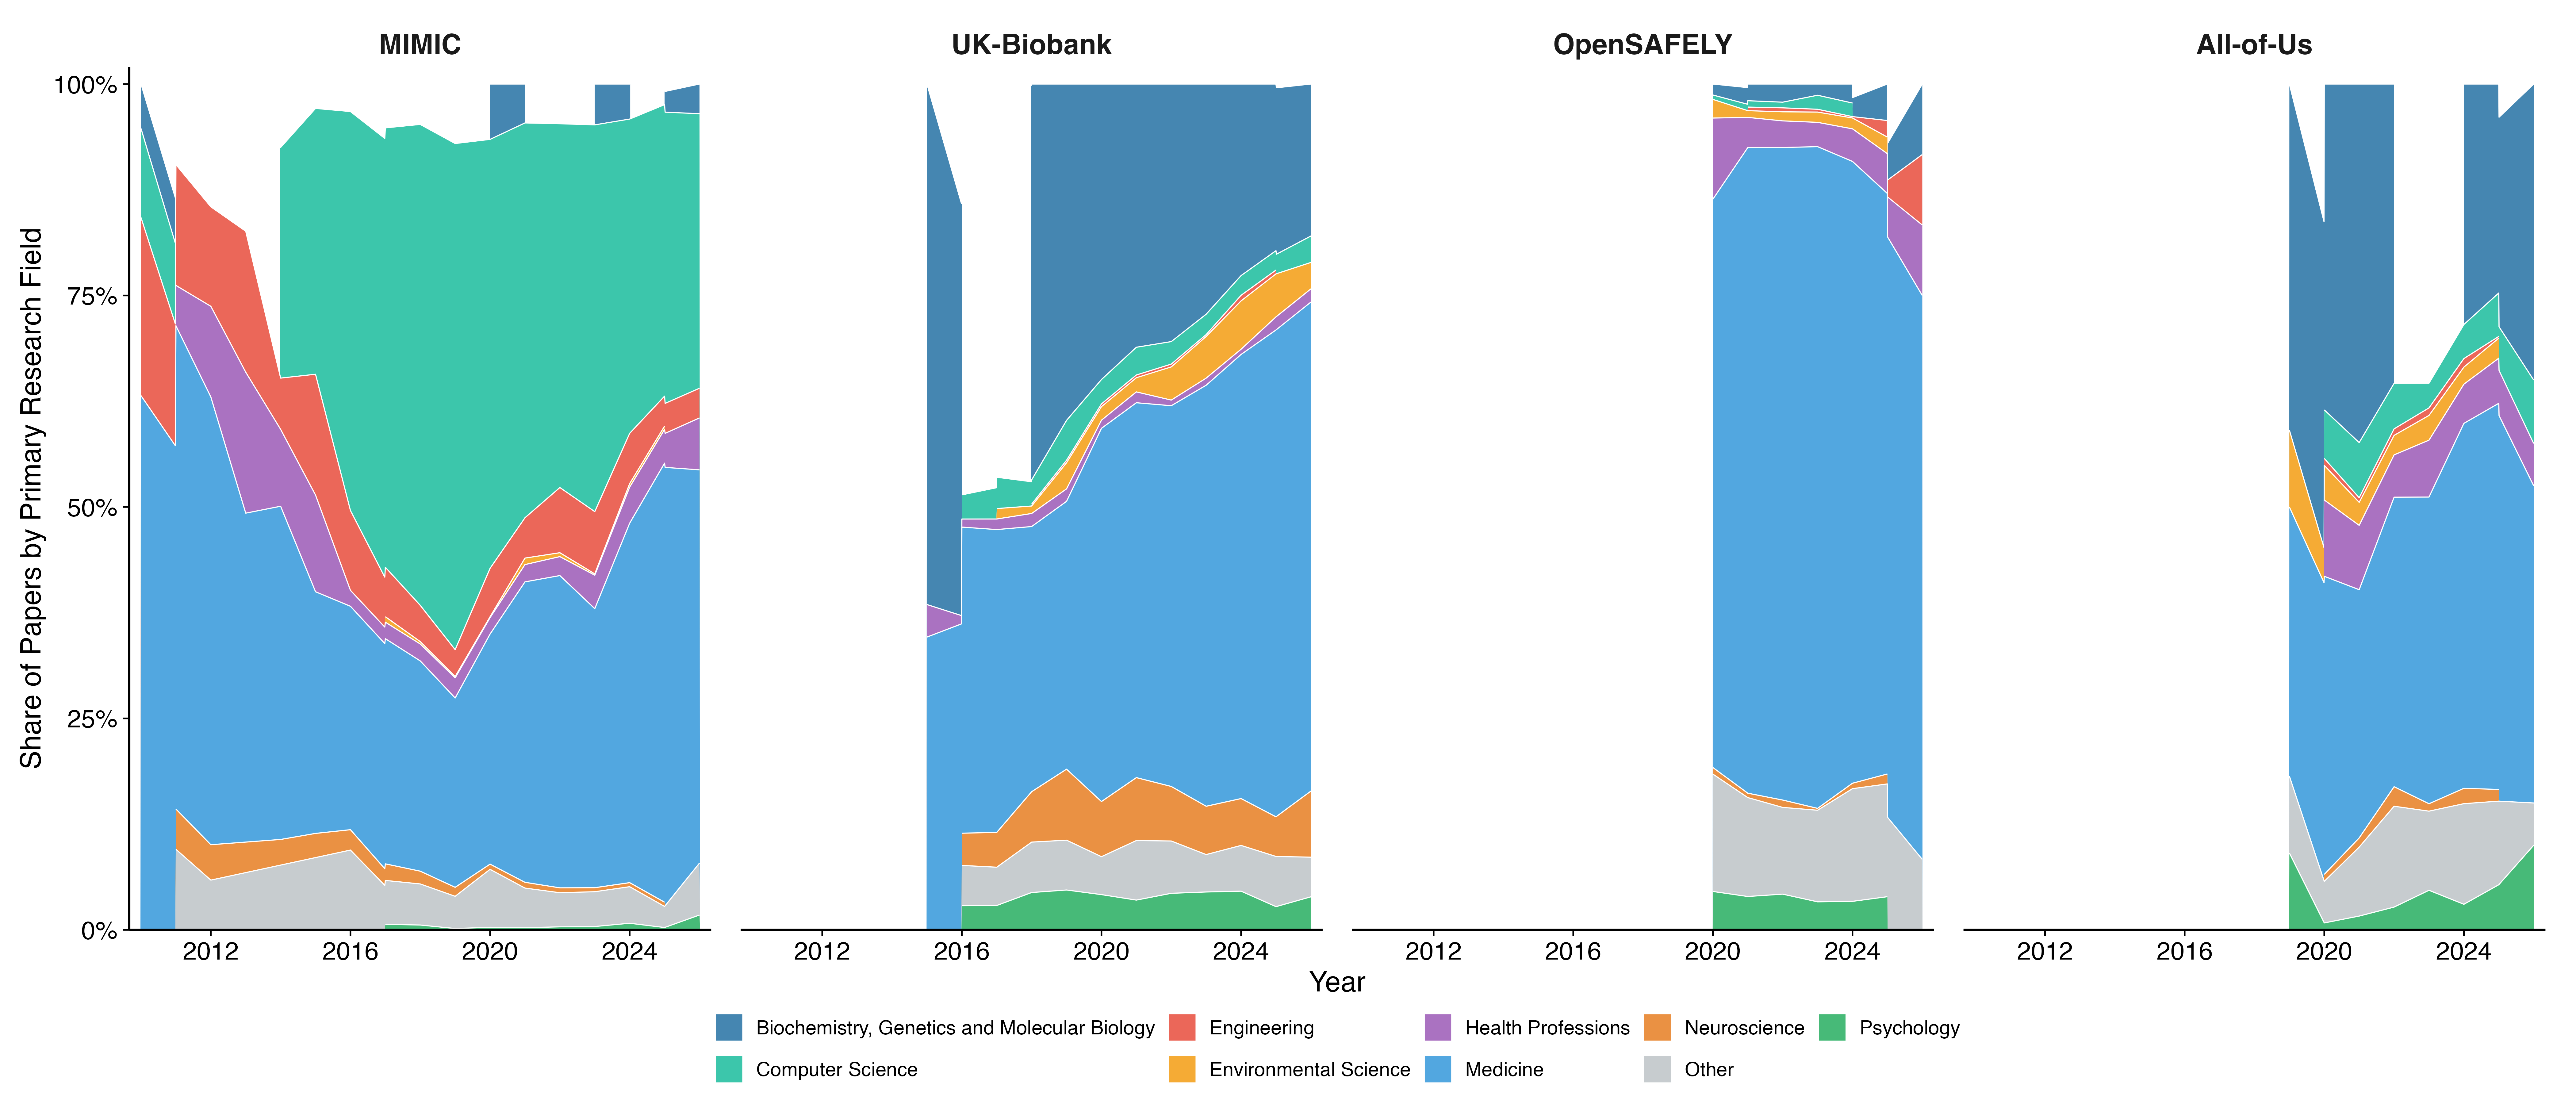
\includegraphics[width=\textwidth]{figures/fig5_disciplinary_diffusion.png}
\caption{Disciplinary composition of first-degree publications over time by repository. Each color represents a research field as classified by OpenAlex. Only year--repository combinations with $\geq$10 papers are shown. MIMIC is the only repository whose primary citing field is computer science (43.1\%) rather than medicine, reflecting its widespread adoption as a machine learning benchmark. UK Biobank is dominated by biochemistry, genetics, and molecular biology. OpenSAFELY and All of Us remain concentrated within medicine.}
\label{fig:disciplines}
\end{figure}

\subsection*{eFigure 2. Citation Distributions}

\begin{figure}[htbp]
\centering

\includegraphics[width=\textwidth]{../figures/figure_2_new.png}
\caption{Citation distributions for first-degree publications. Panel A: Raw citation counts by paper rank (log-log scale). Panel B: Funding-normalized citations per \$1M by paper rank (log-log scale). MIMIC papers are more highly cited per dollar of funding across the full rank distribution.}
\label{fig:citedist}
\end{figure}

\subsection*{eFigure 3. Second-Degree Citation Distributions}

\begin{figure}[htbp]
\centering

\includegraphics[width=\textwidth]{../figures/figure_5_second_degree.png}
\caption{Citation distributions for second-degree publications. Panel A: Raw citation distribution (number of papers at each citation count). Panel B: Funding-normalized citation distribution. The distributions are broadly similar across repositories, consistent with the ${\sim}$10$\times$ amplification constant.}
\label{fig:sddist}
\end{figure}


\subsection*{eTable 1. Pairwise Statistical Comparisons (MIMIC vs.\ Other Repositories)}

\begin{table}[htbp]
\centering
\caption{Pairwise chi-square tests comparing MIMIC with each other repository for LMIC representation and gender distribution. All \textit{p}-values are Bonferroni-corrected ($n = 3$).}
\label{etab:pairwise}
\small
\begin{tabular}{@{}llrccc@{}}
\toprule
\textbf{Comparison} & \textbf{Measure} & $\boldsymbol{\chi^2}$ & \textbf{\textit{p} (adj)} & \textbf{$V$} & \textbf{OR (95\% CI)} \\
\midrule
MIMIC vs.\ UK Biobank & LMIC & 5,527.8 & $<$0.001 & 0.186 & 2.34 (2.29--2.40) \\
MIMIC vs.\ UK Biobank & Gender & 792.7 & $<$0.001 & 0.066 & 0.74 (0.73--0.76) \\
MIMIC vs.\ OpenSAFELY & LMIC & 8,156.3 & $<$0.001 & 0.278 & 3.53 (3.43--3.63) \\
MIMIC vs.\ OpenSAFELY & Gender & 1,317.8 & $<$0.001 & 0.102 & 0.65 (0.64--0.67) \\
MIMIC vs.\ All of Us & LMIC & 9,511.7 & $<$0.001 & 0.378 & 17.71 (16.45--19.07) \\
MIMIC vs.\ All of Us & Gender & 884.3 & $<$0.001 & 0.106 & 0.61 (0.59--0.63) \\
\bottomrule
\end{tabular}

\vspace{4pt}
{\footnotesize OR for LMIC: odds of LMIC authorship in MIMIC relative to comparator (OR $>$1 = higher in MIMIC). OR for gender: odds of female authorship in MIMIC relative to comparator (OR $<$1 = lower in MIMIC).}
\end{table}


\subsection*{eTable 2. Intersectional Analysis: Gender by Income Classification and Authorship Position}

\begin{table}[htbp]
\centering
\caption{Proportion of female authors within HIC and LMIC subgroups, by authorship position. Female representation is consistently higher among LMIC authors than HIC authors across all repositories and positions.}
\label{etab:intersectional}
\small
\begin{tabular}{@{}llcccc@{}}
\toprule
& & \multicolumn{2}{c}{\textbf{HIC Female (\%)}} & \multicolumn{2}{c}{\textbf{LMIC Female (\%)}} \\
\cmidrule(lr){3-4} \cmidrule(lr){5-6}
\textbf{Repository} & \textbf{Position} & \textit{n} & \textbf{\%} & \textit{n} & \textbf{\%} \\
\midrule
MIMIC & First & 1,400 & 30.0 & 1,310 & 36.4 \\
& Middle & 5,089 & 29.1 & 5,081 & 38.4 \\
& Last & 1,109 & 23.9 & 1,044 & 31.9 \\
\midrule
UK Biobank & First & 3,048 & 40.8 & 1,384 & 44.7 \\
& Middle & 26,271 & 37.4 & 9,582 & 44.7 \\
& Last & 2,145 & 29.5 & 926 & 35.3 \\
\midrule
OpenSAFELY & First & 1,777 & 42.6 & 542 & 46.2 \\
& Middle & 16,606 & 42.2 & 3,653 & 46.8 \\
& Last & 1,325 & 34.6 & 400 & 37.5 \\
\midrule
All of Us & First & 745 & 43.1 & 30 & 40.0 \\
& Middle & 6,500 & 43.6 & 281 & 43.4 \\
& Last & 611 & 37.9 & 24 & 48.0 \\
\bottomrule
\end{tabular}
\end{table}


\subsection*{eTable 3. Unique Author Demographics}

\begin{table}[htbp]
\centering
\caption{Unique author demographics by repository. Authors are deduplicated by OpenAlex author ID within each dataset.}
\label{etab:unique}
\small
\begin{tabular}{@{}lcccc@{}}
\toprule
& \textbf{MIMIC} & \textbf{UK Biobank} & \textbf{OpenSAFELY} & \textbf{All of Us} \\
\midrule
Unique authors & 33,573 & 51,783 & 44,441 & 13,238 \\
Female (\%) & 33.5 & 41.3 & 43.7 & 44.4 \\
LMIC (\%) & 47.3 & 30.2 & 21.8 & 5.2 \\
\midrule
Ever first author (\textit{n}) & 6,921 & 7,278 & 4,810 & 1,517 \\
\quad Female (\%) & 32.8 & 42.7 & 43.0 & 43.8 \\
\quad LMIC (\%) & 39.2 & 31.3 & 21.3 & 3.8 \\
\midrule
Ever last author (\textit{n}) & 5,853 & 5,071 & 4,289 & 1,271 \\
\quad Female (\%) & 28.3 & 32.8 & 35.5 & 39.4 \\
\quad LMIC (\%) & 40.7 & 27.0 & 21.5 & 3.3 \\
\bottomrule
\end{tabular}

\vspace{4pt}
{\footnotesize ``Ever first/last author'' = unique authors who held that position on at least one publication citing the repository. MIMIC's unique LMIC authorship (47.3\%) exceeds its record-level rate (41.8\%) because LMIC authors appear on fewer papers on average.}
\end{table}


\end{document}
